% vim:filetype=tex:textwidth=0:linebreak:shiftwidth=4:softtabstop=4:indentexpr=:expandtab
\documentclass[11pt,mathserif,unknownkeysallowed]{beamer}
\usepackage{appendixnumberbeamer}
\usepackage[english]{babel}
\usepackage{booktabs}
\usepackage{changepage}
\usepackage{colortbl}
\usepackage[T1]{fontenc}
\usepackage[latin1]{inputenc}
\usepackage{mathtools}
\usepackage{wasysym}
\usepackage{minibox}
\usepackage{multirow}
\usepackage{qrcode}
\usepackage[full]{textcomp}
\usepackage{xparse}
\usepackage{xcolor}

\usepackage{ubuntu}
\usepackage[default,scale=0.90]{opensans}
\usepackage{charter}

\DeclareSymbolFont{Letters}{U}{zeur}{m}{n}% Euler
\DeclareMathSymbol\Gamma    {\mathalpha}{Letters}{"00}
\DeclareMathSymbol\Delta    {\mathalpha}{Letters}{"01}
\DeclareMathSymbol\Theta    {\mathalpha}{Letters}{"02}
\DeclareMathSymbol\Lambda   {\mathalpha}{Letters}{"03}
\DeclareMathSymbol\Xi       {\mathalpha}{Letters}{"04}
\DeclareMathSymbol\Pi       {\mathalpha}{Letters}{"05}
\DeclareMathSymbol\Sigma    {\mathalpha}{Letters}{"06}
\DeclareMathSymbol\Upsilon  {\mathalpha}{Letters}{"07}
\DeclareMathSymbol\Phi      {\mathalpha}{Letters}{"08}
\DeclareMathSymbol\Psi      {\mathalpha}{Letters}{"09}
\DeclareMathSymbol\Omega    {\mathalpha}{Letters}{"0A}
\DeclareMathSymbol{\alpha}  {\mathalpha}{Letters}{"0B}
\DeclareMathSymbol{\beta}   {\mathalpha}{Letters}{"0C}
\DeclareMathSymbol{\gamma}  {\mathalpha}{Letters}{"0D}
\DeclareMathSymbol{\delta}  {\mathalpha}{Letters}{"0E}
\DeclareMathSymbol{\epsilon}{\mathalpha}{Letters}{"0F}
\DeclareMathSymbol{\zeta}   {\mathalpha}{Letters}{"10}
\DeclareMathSymbol{\eta}    {\mathalpha}{Letters}{"11}
\DeclareMathSymbol{\theta}  {\mathalpha}{Letters}{"12}
\DeclareMathSymbol{\iota}   {\mathalpha}{Letters}{"13}
\DeclareMathSymbol{\kappa}  {\mathalpha}{Letters}{"14}
\DeclareMathSymbol{\lambda} {\mathalpha}{Letters}{"15}
\DeclareMathSymbol{\mu}     {\mathalpha}{Letters}{"16}
\DeclareMathSymbol{\nu}     {\mathalpha}{Letters}{"17}
\DeclareMathSymbol{\xi}     {\mathalpha}{Letters}{"18}
\DeclareMathSymbol{\pi}     {\mathalpha}{Letters}{"19}
\DeclareMathSymbol{\rho}    {\mathalpha}{Letters}{"1A}
\DeclareMathSymbol{\sigma}  {\mathalpha}{Letters}{"1B}
\DeclareMathSymbol{\tau}    {\mathalpha}{Letters}{"1C}
\DeclareMathSymbol{\upsilon}{\mathalpha}{Letters}{"1D}
\DeclareMathSymbol{\phi}    {\mathalpha}{Letters}{"1E}
\DeclareMathSymbol{\chi}    {\mathalpha}{Letters}{"1F}
\DeclareMathSymbol{\psi}    {\mathalpha}{Letters}{"20}
\DeclareMathSymbol{\omega}  {\mathalpha}{Letters}{"21}
\DeclareMathSymbol{\varepsilon}{\mathalpha}{Letters}{"22}
\DeclareMathSymbol{\vartheta}{\mathalpha}{Letters}{"23}
\DeclareMathSymbol{\varpi}  {\mathalpha}{Letters}{"24}
\DeclareMathSymbol{\varphi} {\mathalpha}{Letters}{"27}
\DeclareMathSymbol\upOmega  {\mathord}{Letters}{"0A}
\DeclareMathSymbol\upDelta  {\mathord}{Letters}{"01}

% Logics
\renewcommand\L{\ensuremath{\mathcal{L}}}
\newcommand\LL{\ensuremath{\mathcal{L\mspace{-1mu}L}}}
\newcommand{\plus}{\textsuperscript{+}}
\newcommand\Limbo{\textsc{limbo}}
\newcommand\limbo{\textsc{limbo}}
\newcommand\lb[5]{{\bfseries\color{#1}\bfseries\rotatebox{#2}{\raisebox{#3}{#5}\hspace{#4}}}}
\newcommand\Limboc{{%
\fontUbuntuMedium\itshape%
\lb{limbo1}{-15}{0.35ex}{-0.25em}{L}%
\lb{limbo2}{-20}{0.20ex}{-0.21em}{i}%
\lb{limbo3}{0}{-0.0ex}{-0.17em}{m}%
\lb{limbo4}{10}{-0.05ex}{-0.2em}{b}%
\lb{limbo5}{20}{-0.2ex}{-0.0em}{o}%
}}%
% Operators and operands
\newcommand\e{\mathbin{=}}
\newcommand\n{\mathbin{\neq}}
\newcommand\fa[1]{\forall \mspace{1mu} #1 \mspace{2mu}}
\newcommand\ex[1]{\exists \mspace{1mu} #1 \mspace{2mu}}
\newcommand\limp{\rightarrow}
\newcommand\limped{\leftarrow}
\newcommand\lequiv{\leftrightarrow}
\newcommand\Limped{\mathrel{\texttt{:-}}}
\newcommand\Lquery{\mathrel{\texttt{?-}}}
\newcommand\dneg{\mathrm{not}\,}
%\newcommand\dneg{{\sim}}
\newcommand\lland{\mathrm{,}\,}
\newcommand\llor{\mathrm{;}\,}
\newcommand\Dneg{\texttt{not}\,}
\newcommand\Land{\texttt{,}\,}
\newcommand\lend{\mathrm{.}}
\newcommand\Lend{\texttt{.}}
\newcommand\choice[1]{\{#1\}}
\newcommand\Choice[1]{\texttt{\{}#1\texttt{\}}}
\newcommand\cond[2]{#1\mathrel{:}#2}
\newcommand\Cond[2]{#1\mathrel{\texttt:}#2}
\newcommand\card[3]{#1\mathrel{#2}#3}
\newcommand\Card[3]{#1\mathrel{#2}#3}
\newcommand\Head{\mathrm{Head}}
\newcommand\Body{\mathrm{Body}}
\newcommand\Pos{\mathrm{Pos}}
\newcommand\Neg{\mathrm{Neg}}
\newcommand\dummy{\mathit{dummy}}
\newcommand\entails{\models}
\renewcommand\emptyset{{\{\}}}
\newcommand\modelst[1]{\mathrel{{\mathrel|\joinrel\stackrel{\mathclap{#1}}{=}}}}
\newcommand\entailst[1]{\modelst{#1}}
\newcommand\modelss{\mathrel{{\mathrel|\joinrel\approx}}}
\newcommand\entailss{\modelss}
\newcommand\modelsst[1]{\mathrel{{\mathrel|\joinrel\stackrel{\mathclap{#1}}{\approx}}}}
\newcommand\entailsst[1]{\modelsst{#1}}
\newcommand\Vars{\mathcal{X}}
\newcommand\Names{\mathcal{N}}
\newcommand\Terms{\mathcal{T}}
\newcommand\G{\mathbf{G}\mspace{1mu}}
\newcommand\K[1][]{\mathbf{K}_{#1}\mspace{1mu}}
\newcommand\M[1][]{\mathbf{M}_{#1}\mspace{1mu}}
\newcommand\OO{\mathbf{O}\mspace{1mu}}
\newcommand\Lmod[1][]{\mathbf{L}_{#1}\mspace{1mu}}
\newcommand\Min[1]{#1\textsuperscript{\textminus}}
\newcommand\Max[1]{#1\textsuperscript{+}}
\newcommand\UP[1]{\mathrm{UP}\ifx\uchyph#1\uchyph\else(#1)\fi}
\newcommand\VP[1]{\Max{\mathsf{UP}}\ifx\uchyph#1\uchyph\else(#1)\fi}
\newcommand\WP[1]{\Min{\mathsf{UP}}\ifx\uchyph#1\uchyph\else(#1)\fi}
%\newcommand\flip[1]{\mathrlap{\smash{\overline{\vphantom{\ell}\hphantom{#1}}}}#1}
%\newcommand\flip[1]{\bar{#1}}
\newcommand\flip[1]{\overline{#1}}
\newcommand\gnd{\mathsf{gnd}}
\newcommand\NF{\mathsf{NF}}
\newcommand\BigO{\mathcal{O}}
\newcommand\RES[2]{\mathsf{RES}\ifx\uchyph#1#2\uchyph\else[#1,#2]\fi}
\newcommand\RED[2]{\|#2\|_{\ifx\uchyph#1\uchyph\else#1\fi}}
\newcommand\TRUE{{\normalfont\textsc{true}}}
\newcommand\FALSE{{\normalfont\textsc{false}}}
\newcommand\obj[1]{\ensuremath{\textsuperscript{\raisebox{-0.3\height}{\#}}#1}}
\newcommand\KB{\mathrm{KB}}
\newcommand\CNF{\mathsf{CNF}}
\newcommand\DNF{\mathsf{DNF}}
% Examples
\newcommand\stdname[1]{{\textrm{#1}}}
\newcommand\func[1]{{\textrm{#1}}}
\newcommand\pred[1]{{\textrm{#1}}}
\newcommand\Sally{\stdname{Sally}}
\newcommand\Frank{\stdname{Frank}}
\newcommand\Fred{\stdname{Fred}}
\newcommand\T{\top}
\newcommand\fatherOf{\func{fatherOf}}
\newcommand\rich{\func{rich}}
\newcommand\Rich{\func{Rich}}
%\renewcommand\fatherOf{\func{f}}
%\renewcommand\Rich{\func{R}}
%\renewcommand\rich{\func{r}}
%\renewcommand\Sally{\stdname{S}}
% Dense dots
\newcommand\sldots{\ensuremath{\!\ldotp\!\ldotp\!\ldotp\!}}
% Checkmark
\usepackage{pifont}
\newcommand{\cmark}{\ding{51}}
%\newcommand{\cmark}{\ding{52}}
\newcommand{\xmark}{\ding{55}}
%\newcommand{\xmark}{\ding{56}}
\usepackage{cancel}
\newcommand\strikeout[2][red!50!black]{\setbox0=\hbox{$#2$}%
\rlap{\raisebox{.35\ht0}{\textcolor{#1}{\rule{\wd0}{1pt}}}}#2} 
% Complexity theory
\newcommand\compclass[1]{\ensuremath{\normalfont\textsf{#1}}}
\newcommand\decproblem[1]{\ensuremath{\normalfont\textsf{#1}}}
\renewcommand\P{\compclass{P}}
\newcommand\NP{\compclass{NP}}
\newcommand\PSPACE{\compclass{PSPACE}}
\newcommand\SAT{\decproblem{SAT}}
\newcommand\kSAT[1]{\decproblem{#1-SAT}}
%\newcommand\mreducible[1][]{\ensuremath{\reducible_{\mathrm{m}}^{\mathrm{#1}}}}
\newcommand\mpreducible{\ensuremath{\leqq_{\P}}}

\usepackage{ulem}
\normalem % use classical emph
\usepackage{pgffor}
\newcommand\myul[5][white]{% arg 1: background color; arg 2: underline depth; arg 3: underline thickness; arg 4: space around descenders in ex (!); arg 5: text
  \begingroup%
  \renewcommand\ULdepth{#2}%
  \renewcommand\ULthickness{#3}%
  \uline{\phantom{\smash{#5}}}%
  \pgfmathparse{#4 / 5.0}%
  \foreach \hshift in {0.0, \pgfmathresult, ..., #4}{%
    \foreach \upshift in {0.0, 0.1, ..., 1.0}{%
      \llap{\color{#1}\raisebox{\upshift0pt}[0pt]{#5}\hspace{\hshift0em}}%
      \llap{\color{#1}\raisebox{\upshift0pt}[0pt]{#5}\hspace{-\hshift0em}}%
    }%
  }%
  \llap{#5}%
  \endgroup%
}
\newcommand<>\important[2][white]{\alt#3{\myul[#1]{.35ex}{.1ex}{0.12}{#2}}{#2}}
\newcommand<>\muline[1]{\alt#2{\blue{\uwave{\hphantom{#1}}}\mathllap{#1}}{#1}}

\DeclareDocumentCommand{\mybox}{ O{structure} O{0.3ex} O{1.5ex} O{0.0ex} m }{%
    \setlength{\fboxrule}{#2}%
    \setlength{\fboxsep}{#3}%
    \fcolorbox{#1}{white}{\hspace{#4}\minibox{#5}\hspace{#4}}%
}%

% Tikz
\usepackage{tikz}
\usepackage{pgfplots}
\usetikzlibrary{arrows,calc,decorations,decorations.pathmorphing,decorations.pathreplacing,shapes.misc,fit,patterns,positioning}

\definecolor{darkred}{rgb}{0.9,0.1,0.1}
\definecolor{darkblue}{rgb}{0.2,0.2,0.7}
\definecolor{darkgreen}{rgb}{0.2,0.7,0.2}
\definecolor{babyblue}{rgb}{0.5,0.5,1.0}
\definecolor{deeppink}{HTML}{FF1493}
\definecolor{realpurple}{HTML}{800080}
\definecolor{limbo1}{HTML}{2020D0} % slightly darker blue
\definecolor{limbo2}{HTML}{FF0000} % red
\definecolor{limbo3}{HTML}{FFD000} % gold
\definecolor{limbo4}{HTML}{00BB00} % green!80!black
\definecolor{limbo5}{HTML}{800080} % realpurple
\newcommand\hicolor{darkblue}
\newcommand\locolor{babyblue}
\newcommand<>\hi[1]{{{}\color#2{\hicolor}#1}}
\newcommand<>\lo[1]{{{}\color#2{\locolor}#1}}
\newcommand<>\red[1]{{{}\color#2{darkred}#1}}
\newcommand<>\blue[1]{{{}\color#2{darkblue}#1}}
\newcommand<>\babyblue[1]{{{}\color#2{babyblue}#1}}
\newcommand<>\green[1]{{{}\color#2{darkgreen}#1}}
\newcommand<>\lightgreen[1]{{{}\color#2{darkgreen!45}#1}}
\newcommand<>\yellow[1]{{{}\color#2{yellow!80!black}#1}}
\newcommand<>\orange[1]{{{}\color#2{orange}#1}}
\newcommand<>\purple[1]{{{}\color#2{realpurple}#1}}
\newcommand<>\babypurple[1]{{{}\color#2{realpurple!50}#1}}
\newcommand<>\gray[1]{{{}\color#2{gray!50}#1}}
\newcommand<>\darkgray[1]{{{}\color#2{gray}#1}}
\newcommand<>\pink[1]{{{}\color#2{deeppink}#1}}
\newcommand<>\shadow[1]{{{}\only#2{\setbeameritemcolor{gray!50}\renewcommand<>\hi[1]{####1}}\color#2{gray!50}#1}}
\newcommand\plainmeans{\hat=}
\newcommand\means{\mathrel{\purple{\plainmeans}}}
\newcommand\defeq{\mathrel{\overset{\mathclap{\text{\tiny def}}}{=}}}
\newcommand\opt[1]{\darkgray{(}#1\darkgray{)}}

\newenvironment{defi}[1]{\setbeamercolor{block title}{use=darkblue,fg=white,bg=darkblue}\begin{block}{\smash{#1}\vphantom{X}}}{\end{block}} \newenvironment{recall}[1]{\setbeamercolor{block title}{use=gray!50!white,fg=black,bg=gray!50!white}\begin{block}{\smash{#1}\vphantom{X}}\setbeameritemcolor{gray!50!white}}{\end{block}} \newenvironment{thm}[1]{\setbeamercolor{block title}{use=darkgreen,fg=white,bg=darkgreen}\begin{block}{\smash{#1}\vphantom{X}}\setbeameritemcolor{darkgreen}}{\end{block}} \newenvironment{hienv}[1]{\setbeamercolor{block title}{use=\hicolor,fg=white,bg=\hicolor}\begin{block}{\smash{#1}\vphantom{X}}\setbeameritemcolor{\hicolor}}{\end{block}}

\newcommand\setlohi[3][white]{
%\renewcommand\locolor{#2}%
%\renewcommand\hicolor{#3}%
%\setbeamercolor{frametitle}{bg=#3,fg=#1}%
%\setbeamerfont{frametitle}{series=\bfseries}
%\setbeameritemcolor{#3}%
%\setbeamersubitemcolor{#2}%
}%

\newcommand\singlenode[3][]{%
\tikz[remember picture]%
\node[inner xsep=0pt,inner ysep=0pt,left,#1] (#2) {#3};%
}

\newcommand\internode[2][]{%
\tikz[remember picture,overlay,baseline=(#2.base)]%
\node[inner xsep=0pt,left] (#2) {\phantom{}};%
}

\newcommand<>\fly[2][\textwidth]{%
\only#3{%
\tikz[remember picture,overlay,baseline=(char.base),overlay]%
\node[anchor=south west,inner xsep=0pt,inner ysep=0,right,text width=#1] (char) {
    \begin{minipage}[t][2em]{#1}%
    #2%
    \end{minipage}
    };%
}}%

\newlength\myhighlightsep
\newcommand<>\highlight[2]{%        % \highlight[<colour>]{<text>}
  \setlength{\myhighlightsep}{1.5pt}%
  \setlength{\fboxrule}{0pt}%
  \alt#3{%
  \mathchoice%
  {\setlength{\fboxsep}{\myhighlightsep}\colorbox{#1}{\hspace{-\myhighlightsep}$\displaystyle#2$\hspace{-\myhighlightsep}}}%
  {\setlength{\fboxsep}{\myhighlightsep}\colorbox{#1}{\hspace{-\myhighlightsep}$\textstyle#2$\hspace{-\myhighlightsep}}}%
  {\setlength{\fboxsep}{\myhighlightsep}\colorbox{#1}{\hspace{-\myhighlightsep}$\scriptstyle#2$\hspace{-\myhighlightsep}}}%
  {\setlength{\fboxsep}{\myhighlightsep}\colorbox{#1}{\hspace{-\myhighlightsep}$\scriptscriptstyle#2$\hspace{-\myhighlightsep}}}%
  }{%
  \mathchoice%
  {\setlength{\fboxsep}{\myhighlightsep}\fbox{\hspace{-\myhighlightsep}$\displaystyle#2$\hspace{-\myhighlightsep}}}%
  {\setlength{\fboxsep}{\myhighlightsep}\fbox{\hspace{-\myhighlightsep}$\textstyle#2$\hspace{-\myhighlightsep}}}%
  {\setlength{\fboxsep}{\myhighlightsep}\fbox{\hspace{-\myhighlightsep}$\scriptstyle#2$\hspace{-\myhighlightsep}}}%
  {\setlength{\fboxsep}{\myhighlightsep}\fbox{\hspace{-\myhighlightsep}$\scriptscriptstyle#2$\hspace{-\myhighlightsep}}}%
  }%
  }%
\makeatletter
\newcommand\fullwidth[1]{%
\hspace*{-\beamer@leftmargin}%
\begin{minipage}{\paperwidth}{#1}\end{minipage}%
}
\makeatother
\newcommand\setbeameritemcolor[2][$\blacksquare$]{
    \setbeamercolor*{enumerate item}{fg=#2}
    \setbeamertemplate{itemize item}{{\color{#2}\footnotesize#1}}
}
\newcommand\setbeamersubitemcolor[2][$\blacktriangleright$]{
    \setbeamercolor*{enumerate subitem}{fg=#2}
    \setbeamertemplate{itemize subitem}{{\color{#2}\small#1}}
}
\mode<presentation>{
    \setbeamercolor*{darkblue}{fg=darkblue}
    \setbeamercolor*{alerted text}{fg=darkred}
    \setbeamerfont{title}{size=\LARGE}
    %\setbeamerfont{subtitle}{size=\Large\normalfont\slshape}
    %\setbeamerfont{author}{size=\Large}
    %\setbeamerfont{institute}{size=\normalsize}
    %\setbeamertemplate{frametitle}[default][ht=0ex,dp=0.5ex]
    \setbeamertemplate{headline}{}
    \setbeamertemplate{footline}{
        \begin{beamercolorbox}[wd=\paperwidth,ht=0ex,dp=0.75ex,right]{footline}%
        \slidefooter
        \hspace{.5ex}\parbox{\widthof{00 / 00}}{\hfill \insertframenumber\ / \inserttotalframenumber}\;\;\hspace{.5ex}%
        \end{beamercolorbox}%
    }
    \setbeamertemplate{navigation symbols}{}
    \setbeamertemplate{blocks}[default]
    \setbeamercolor{title}{fg=babyblue}
    \setbeamercolor{frametitle}{fg=darkblue}
    \setbeamercolor{footline}{fg=darkblue,bg=white}
    \setbeamercolor{block body alerted}{bg=normal text.bg!90!black}
    \setbeamercolor{block body}{bg=normal text.bg!90!black}
    \setbeamercolor{block body example}{bg=normal text.bg!90!black}
    \setbeamercolor{block title alerted}{use={normal text,alerted text},fg=alerted text.fg!75!normal text.fg,bg=normal text.bg!75!black}
    \setbeamercolor{block title}{bg=darkblue,fg=white}
    \setbeamercolor{block title example}{use={normal text,example text},fg=example text.fg!75!normal text.fg,bg=normal text.bg!75!black}
    \setbeameritemcolor{darkblue}
    \setbeamertemplate{itemize subitem}{\orange{\small$\blacktriangleright$}}
    \setbeamertemplate{itemize subsubitem}{\yellow{$\bullet$}}
}
\AtBeginSection[]{\begin{frame}<beamer>{Outline} \tableofcontents[currentsection] \end{frame}}
\newcommand\slidefooter{}
%\setbeamersize{text margin left=2em,text margin right=2pt} % beamer margin
\begin{document}

\title{\hi{Satisfiability}}

\author{Christoph~Schwering}
%\institute{c.schwering@unsw.edu.au}
\date{COMP4418, Week 6 \& 7}

\begin{frame}[plain]
\titlepage
\end{frame}

\begin{frame}[t]{The \emph{Reasoning} in KRR}
We've touched \blue{reasoning} a few times so far:
\begin{itemize}
\item On a theoretical level:
    \begin{itemize}
    \item Resolution
        \begin{itemize}
        \item Prove that $\KB$ entails $\psi$ by deriving contradiction from $\KB \land \neg \psi$.
        \item Downside: Difficult to guide search towards goal.
        \end{itemize}
    \item Prolog
        \begin{itemize}
        \item Uses restricted version of resolution.
        \item Downside: More programming than reasoning.
        \end{itemize}
    \end{itemize}
\pause
\item From a user perspective:
    \begin{itemize}
    \item Answer Set Programming
    \item Satisfiability \; {\footnotesize (in Assignment 1, Question 3)}
    \end{itemize}
\end{itemize}

\pause
\bigskip
Today: \blue{propositional reasoning}
\begin{itemize}
\item What algorithms?
\item What do real-world implementations look like?
\item Which problems can be solved using it (in theory \& practice)?
\end{itemize}
\end{frame}

\begin{frame}{Satisfiability}
\begin{defi}{Definition: SAT}
Input: Propositional formula in CNF.\\
Problem: Is this formula satisfiable?
\end{defi}
\bigskip
\begin{itemize}
\item Many problems can be reduced to SAT.
\item In theory, SAT is very difficult.
\item In practice, SAT is often feasible.
\item SAT is extremely important for theory \emph{and} practice.
\end{itemize}

\bigskip
This lecture: only propositional logic.
\end{frame}

\begin{frame}{This Lecture}
The goal of this lecture is twofold:
\bigskip
\begin{itemize}
\item Practical aspects:
    \begin{itemize}
    \item What are data structures / algorithms for SAT solving?
    \item What does an implementation of a SAT solver look like?
    %\item That's pretty close to the state of the art
    \end{itemize}
\bigskip
\item Theoretical aspects:
    \begin{itemize}
    \item Why is SAT hard?
    \item Why is it so important?
    \end{itemize}
\end{itemize}
\end{frame}

\begin{frame}[t]{Impact of Advanced Algorithms}
\vspace{-5ex}
\only<1>{\begin{adjustwidth}{-4em}{-3em}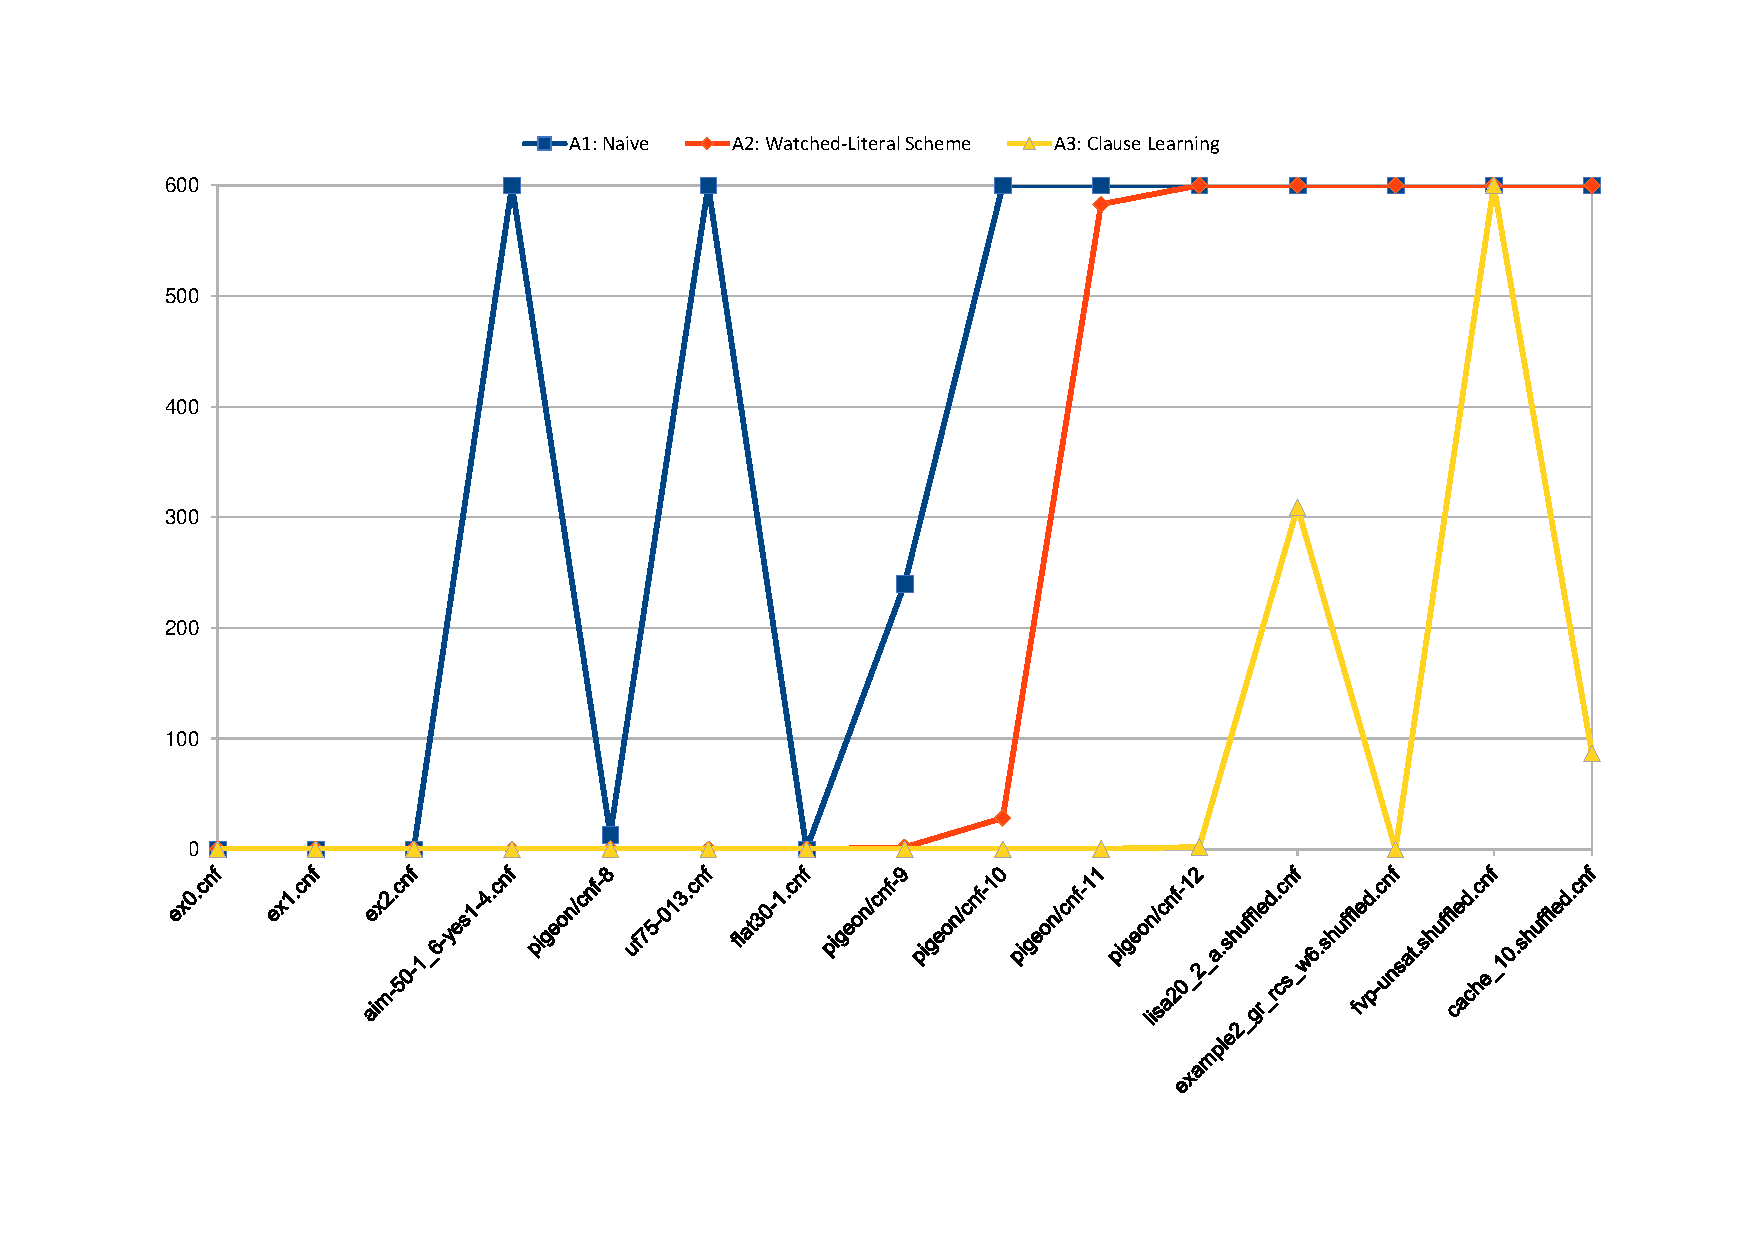
\includegraphics[width=1.2\textwidth]{./benchmark-times.pdf}\end{adjustwidth}}%
\only<2>{\begin{adjustwidth}{-4em}{-3em}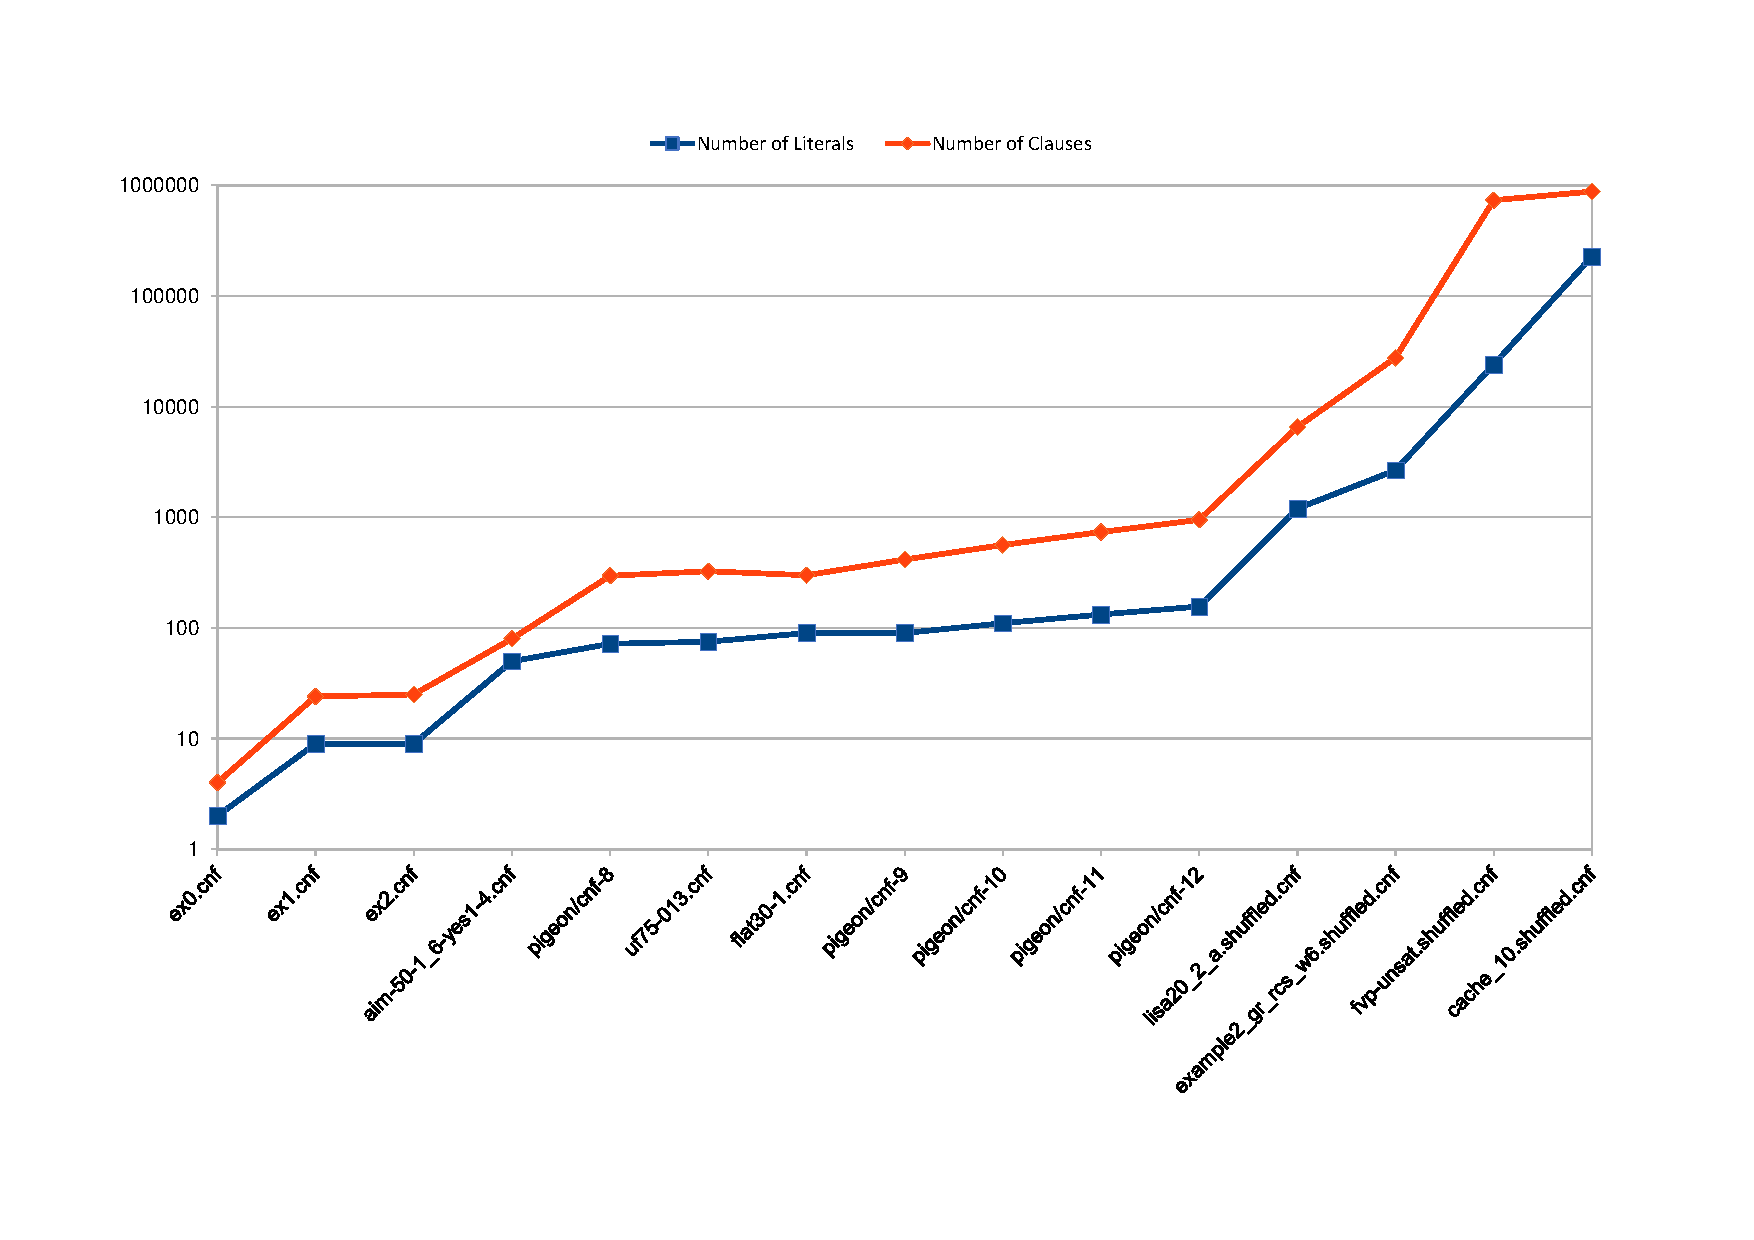
\includegraphics[width=1.2\textwidth]{./benchmark-sizes.pdf}\end{adjustwidth}}%
\vspace{-6.5ex}
\begin{center}
\only<1>{Running times (in seconds) of algorithms for different instances.\vphantom{g}}%
\only<2>{Size of the instances.}%
\end{center}
\end{frame}

\begin{frame}{Outline} \tableofcontents \end{frame}

\section{Satisfiability and Complexity Theory}

\begin{frame}{Propositional Logic}
Syntax:
\begin{itemize}
\item Atomic propositions a.k.a. \blue{variables}.
\item Negation: $\neg \phi$
\item Disjunction: $(\phi_1 \lor \phi_2)$
\item Conjunction: $(\phi_1 \land \phi_2)$
\shadow{\item $\TRUE$, $\FALSE$, $\limp$, $\lequiv$ can be expressed with $\neg, \lor, \land$.}
\end{itemize}
\bigskip

Semantics:
\begin{itemize}
\item An interpretation $I$ maps each variable to true or false.
\item It satisfies $\neg \phi$ \;iff\; it falsifies\footnote{falsify = do not satisfy} $\phi$.
\item It satisfies $(\phi_1 \lor \phi_2)$ \;iff\; it satisfies $\phi_1$ or $\phi_2$.
\item It satisfies $(\phi_1 \land \phi_2)$ \;iff\; it satisfies $\phi_1$ and $\phi_2$.
\end{itemize}
\end{frame}

\begin{frame}{Satisfiability and Validity}
\begin{itemize}
\item $\phi$ is satisfiable \;iff\; some interpretation satisfies $\phi$\\
    \uncover<2->{~\phantom{$\phi$ is satisfiable}\;iff\; not: not: some interpretation satisfies $\phi$\\}
    \uncover<3->{~\phantom{$\phi$ is satisfiable}\;iff\; not: all interpretations falsify $\phi$\\}
    \uncover<4->{~\phantom{$\phi$ is satisfiable}\;iff\; not: all interpretations satisfy $\neg \phi$\\}
    \uncover<5->{~\phantom{$\phi$ is satisfiable}\;iff\; $\neg \phi$ is not valid}
\bigskip
\item $\phi$ is valid \;iff\; all interpretations satisfy $\phi$\\
    \uncover<6->{~\phantom{$\phi$ is valid}\;iff\; not: not: all interpretation satisfy $\phi$\\}
    \uncover<7->{~\phantom{$\phi$ is valid}\;iff\; not: some interpretation falsifies $\phi$\\}
    \uncover<8->{~\phantom{$\phi$ is valid}\;iff\; not: some interpretation satisfies $\neg \phi$\\}
    \uncover<9->{~\phantom{$\phi$ is valid}\;iff\; $\neg \phi$ is not satisfiable}
\end{itemize}
\end{frame}

\begin{frame}[t]{Disjunctive Normal Form}
\bigskip
\begin{defi}{Definition: DNF}
A formula $\psi$ is in Disjunctive Normal Form iff\\
~\qquad $\psi$ is of the form $(d_1 \lor \ldots \lor d_k)$, where each\\
~\qquad $d_i$ is of the form $(x_{i1} \land \ldots \land x_{i{l_i}})$, where each\\
~\qquad $x_{ij}$ is a literal.
\end{defi}

\bigskip
\important{Ex.}: $(p \land q) \lor (\neg p \land \neg q) \lor (p \land \neg q \land r) \lor (\neg p \land q \land r)$

\bigskip
Every formula can be converted into an equivalent formula in DNF.
{\small (Convert into NNF, then use transitivity and distributivity of $\land$ and $\lor$.)}

\bigskip
\important{Note}: Satisfiability for DNF is very easy {(solvable in linear time)}.
\end{frame}

\begin{frame}[t]{Conjunctive Normal Form}
\bigskip
\begin{defi}{Definition: CNF}
A formula $\phi$ is in Conjunctive Normal Form iff\\
~\qquad $\phi$ is of the form $(c_1 \land \ldots \land c_k)$, where each\\
~\qquad $c_i$ is of the form $(x_{i1} \lor \ldots \lor x_{i{l_i}})$, where each\\
~\qquad $x_{ij}$ is a literal.
\end{defi}

\bigskip
\important{Ex.}: $(\neg p \lor \neg q) \land (p \lor q) \land (\neg p \lor q \lor \neg r) \land (p \lor \neg q \lor \neg r)$

\bigskip
Every formula can be converted into an equivalent formula in CNF.
{\small (Convert into NNF, then use transitivity and distributivity of $\land$ and $\lor$.)}

\bigskip
\important{Note}: Validity for CNF is very easy {(solvable in linear time)}.
\end{frame}

\begin{frame}{SAT and CNF}
\begin{defi}{Definition: SAT}
Input: $\phi$ in CNF.\\
Problem: Is this formula satisfiable?
\end{defi}

\bigskip

Why not DNF?
\begin{itemize}
\item Satisfiability for DNF is very easy, but \ldots
\item DNF of formula may grow exponentially!
\end{itemize}

\bigskip

Why CNF?
\begin{itemize}
\item Structure of CNF is much simpler than of arbitrary formulas.
\item Every formula $\psi$ can be transformed to a formula $\phi$ such \rlap{that:}
    \begin{itemize}
    \item $\phi$ is satisfiable iff $\psi$ is satisfiable.
    \item The size of $\phi$ is linear in the size of $\psi$.
    \end{itemize}
\end{itemize}
\end{frame}

\begin{frame}{Tseitin transformation: Example}
Input: $\psi = (\neg ((p \lor q) \land r) \lor \neg s)$
\pause
\begin{align*}
& (\neg ((p \lor q) \land r) \lor \neg s)\\
& \uncover<-8>{\phantom{(\neg ((}p\phantom{{} \lor q) \land r) \lor \neg s)}}    &\only<9->{\mathllap{\phi ={}}}& \alt<10->{(\neg x_1 \lor p) \land (x_1 \lor \neg p)}{\uncover<9->{\CNF[}\uncover<3->{x_1 \lequiv p}\uncover<9->{]}}\\
& \uncover<-8>{\phantom{(\neg ((p \lor{}} q\phantom{) \land r) \lor \neg s)}}    &\uncover<9->{{}\land{}}          & \alt<10->{(\neg x_2 \lor q) \land (x_2 \lor \neg q)}{\uncover<9->{\CNF[}\uncover<3->{x_2 \lequiv q}\uncover<9->{]}}\\
& \uncover<-8>{\phantom{(\neg ((p \lor q) \land{}} r\phantom{) \lor \neg s)}}    &\uncover<9->{{}\land{}}          & \alt<10->{(\neg x_3 \lor r) \land (x_3 \lor \neg r)}{\uncover<9->{\CNF[}\uncover<3->{x_3 \lequiv r}\uncover<9->{]}}\\
& \uncover<-8>{\phantom{(\neg ((p \lor q) \land r) \lor \neg} s\phantom{)}}      &\uncover<9->{{}\land{}}          & \alt<10->{(\neg x_4 \lor s) \land (x_4 \lor \neg s)}{\uncover<9->{\CNF[}\uncover<3->{x_4 \lequiv s}\uncover<9->{]}}\\
& \uncover<-8>{\phantom{(\neg ((p \lor q) \land r) \lor{}} \neg s\phantom{)}}    &\uncover<9->{{}\land{}}          & \alt<10->{(\neg x_5 \lor \neg x_4) \land (x_5 \lor \neg x_4)}{\uncover<9->{\CNF[}\uncover<3->{x_5 \lequiv \alt<4>{\neg x_4}{\neg s}}\uncover<9->{]}}\\
& \uncover<-8>{\phantom{(\neg (}(p \lor q) \phantom{{}\land r) \lor \neg s)}}    &\uncover<9->{{}\land{}}          & \alt<10->{(\neg x_6 \lor x_1 \lor x_2) \land (x_6 \lor \neg x_1) \land (x_6 \lor \neg x_2)}{\uncover<9->{\CNF[}\uncover<3->{x_6 \lequiv \alt<5->{(x_1 \lor x_2)}{(p \lor q)}}\uncover<9->{]}}\\
& \uncover<-8>{\phantom{(\neg} ((p \lor q) \land r) \phantom{{}\lor \neg s)}}    &\uncover<9->{{}\land{}}          & \alt<10->{(\neg x_7 \lor x_6) \land (\neg x_7 \lor x_3) \land (x_7 \lor \neg x_6 \lor \neg x_3)}{\uncover<9->{\CNF[}\uncover<3->{x_7 \lequiv \alt<6->{(x_6 \land x_3)}{((p \lor q) \land r)}}\uncover<9->{]}}\\
& \uncover<-8>{\phantom{(}\neg ((p \lor q) \land r) \phantom{{}\lor \neg s)}}    &\uncover<9->{{}\land{}}          & \alt<10->{(\neg x_8 \lor \neg x_7) \land (x_8 \lor x_7)}{\uncover<9->{\CNF[}\uncover<3->{x_8 \lequiv \alt<7->{\neg x_7}{\neg ((p \lor q) \land r)}}\uncover<9->{]}}\\
& \uncover<-8>{(\neg ((p \lor q) \land r) \lor \neg s)}                          &\uncover<9->{{}\land{}}          &\alt<10->{(\neg x_9 \lor x_8 \lor x_5) \land (x_9 \lor \neg x_8) \land (x_9 \lor \neg x_5)}{\uncover<9->{\CNF[}\uncover<3->{x_9 \lequiv \alt<8->{(x_8 \lor x_5)}{(\neg ((p \lor q) \land r) \lor \neg s)}}\uncover<9->{]}}\\
&                                                                                &\uncover<9->{{}\land{}}          &\uncover<9->{\mathrlap{x_9}}\qquad\qquad\qquad\qquad\qquad\qquad\qquad\qquad\qquad\qquad\quad
\end{align*}
\end{frame}

\begin{frame}{Tseitin Transformation}
Input: formula $\psi$. \; Output: formula $\phi$ in CNF.
\begin{itemize}
\item Let $\rho_1,\ldots,\rho_k$ be all sub-formulas of $\psi$, where $\rho_k = \psi$.
\item Let $x_1,\ldots,x_k$ be fresh variables.
\item Let $\phi = \CNF[x_1 \lequiv f(\rho_1)] \land \ldots \land \CNF[x_k \lequiv f(\rho_k)] \land x_k$ where
    \begin{itemize}
    \item $f(\rho_i \land \rho_j) = (x_i \land x_j)$
    \item $f(\rho_i \lor \rho_j) = (x_i \lor x_j)$
    \item $f(\neg \rho_i) = \neg x_i$
    \item $f(\rho_i) = x_i$ if $\rho_i$ is a variable.
    \end{itemize}
\end{itemize}

\bigskip
\pause
\begin{thm}{Theorem: Tseitin transformation}
$\phi$ is satisfiable iff $\psi$ is satisfiable.\\
$\phi$ is in 3-CNF and its size is linear in the size of $\psi$.
\end{thm}

\bigskip
{\small
Why?
The number of subformulas of $\psi$ is at most twice the length $\psi$.\\
The size of $f(\rho_i)$ is constant.
The size of $\CNF[x_i \lequiv f(\rho_i)]$ is constant.
}
\end{frame}

\begin{frame}{Syntax and Semantics Revisited}
Syntax:
\begin{itemize}
\item A CNF formula $\phi$ is of the form $(c_1 \land \ldots \land c_k)$,\\
    where each $c_i$ is of the form $(x_{i1} \lor \ldots \lor x_{il_i})$\\
    where each $x_{ij}$ is a variable or a negated variable.
\item We identify $c_i$ with the set $\{x_{i1},\ldots,x_{il_i}\}$.
\item We identify $\phi$ with the set $\{c_1,\ldots,c_k\}$.
\item We write $\flip x$ to flip the negation of a literal $x$:
    \hfill $\flip{\neg p} = p$
    \hfill $\flip p = \neg p$
\end{itemize}
\bigskip
\pause
Semantics:
\begin{itemize}
\item A partial interpretation $I$ is a consistent set of literals \rlap{($x \notin I$ or $\flip x \notin I$)}\\
      It may falsify or satisfy a formula or neither (because it is \rlap{partial)}
\item $I$ satisfies a CNF formula $\phi$ \;iff\; $I$ satisfies all clauses $c \in \phi$\\
      $I$ falsifies a CNF formula $\phi$ \;iff\; $I$ falsifies some clause $c \in \phi$
\item $I$ satisfies a clause $c$ \;iff\; $I$ satisfies some literal $x \in c$\\
      $I$ falsifies a clause $c$ \;iff\; $I$ falsifies all literals $x \in c$
\item $I$ satisfies a literal $x$ \;iff\; $x \in I$\\
      $I$ falsifies a literal $x$ \;iff\; $\flip x \in I$
\end{itemize}
\end{frame}

\begin{frame}{SAT Algorithm 1a: Nondeterministic}
Let $I = \emptyset$.
Repeat:
\begin{enumerate}
\item If $I$ falsifies some $c \in \phi$: \; return NO
\item Select a variable $x$ such that $x, \flip x \notin I$
\item If there is none: \; return YES
\item Let $I = I \cup \{x\}$ \red<2->{or} $I = I \cup \{\neg x\}$
\end{enumerate}

\pause
\bigskip
\important{Bad news}: \; Search space is exponential in number of variables.\\% \rlap{$\BigO(2^{\text{\#vars}})$}\\
~\phantom{\important{Bad news}:}\; (It is believed that) we can't do better.
\end{frame}

\begin{frame}{Complexity Theory: Big O Notation}
\begin{itemize}
\item Complexity is (usually) measured in the length $n$ of the input:
    \begin{itemize}
    \item $f(n) = \BigO(g(n))$ iff for some $k$, for large $n$, $f(n) \leq k \cdot g(n)$
        \tikz[overlay,remember picture] \node[anchor=north] (growth) at (-.5,-.2) {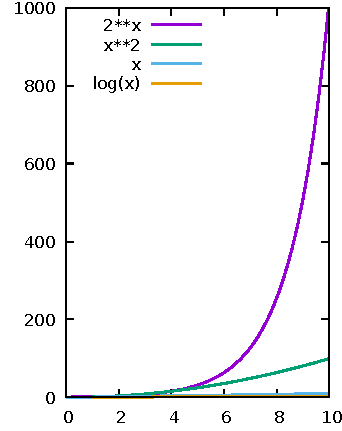
\includegraphics[height=17em]{./growth-3.pdf}};
    \item Exponential complexity: \; $\BigO(k^n)$     %\hfill\rlap{very expensive}\phantom{blablablablablablablablabl}
    \item Polynomial complexity: \;\; $\BigO(n^k)$    %\hfill\rlap{efficient}\phantom{blablablablablablablablabl}
    \item Linear complexity: \qquad\quad\,$\BigO(n)$  %\hfill\rlap{cheap}\phantom{blablablablablablablablabl}
    \item Logarithmic complexity: \;\;$\BigO(\log n)$ %\hfill\rlap{very cheap}\phantom{blablablablablablablablabl}
    \item Constant complexity: \quad\;\; $\BigO(1)$   %\hfill\rlap{free}\phantom{blablablablablablablablabl}
    \end{itemize}
\bigskip
\medskip
\item Length of input $=$ number of symbols:
    \begin{itemize}
    \item Length of ``$\neg (p \land q)$'' $=$ $6$
    \item Length of $173$ in decimal $=$ $3$
    \item Length of $173$ in binary $=$ $8$
    \end{itemize}
    %It's about the length of the representation
\bigskip
\medskip
\item Time complexity: number of computation steps.
\item Space complexity: amount of memory used.
\item Time is upper bound for space.
\end{itemize}
\end{frame}

\begin{frame}[t]{Complexity Theory: \P\ and \NP}
\begin{defi}{Definition: decision problem, complexity class}
A \blue{decision problem} is a yes/no question over a set of instances.\\
An \blue{instance} is a finite sequence of symbols from finite alphabet.\\
A \blue{complexity class} is a set of decision problems of related \rlap{complexity.}
\end{defi}

\pause
\bigskip

\begin{defi}{Definition: complexity class \P, \NP}
$A \in \P\phantom{N}$ \;iff\; solvable in poly. time by a deterministic machine.\\
$A \in \NP$ \;iff\; solvable in poly. time by a nondeterministic machine.
\end{defi}

\begin{itemize}
\item Det. machine takes a predetermined action in each state.
\item Nondet. m. takes \blue{one out of a set of possible actions} \rlap{in each state.}
    \begin{itemize}
    \item The machine \orange{guesses} which \orange{action} to take.
    \item The machine guesses the shortest way to \orange{``yes''} if there is one.
    \end{itemize}
\end{itemize}

\pause
\bigskip

\begin{thm}{Theorem: alternative characterisation of \NP}
$A \in \NP$ \;iff\; ``yes''-proof verifiable by a det.\ machine in poly.\ time.
\end{thm}
\end{frame}

\begin{frame}{Complexity Theory: \NP-Completeness}
A problem is \NP-complete if it's among the hardest problems \rlap{in \NP.}

\pause
\bigskip
\begin{defi}{Definition: reduction from $A$ to $B$}
$A \mpreducible B$ \;iff\; for some function $f$ from $A$-instances to $B$-instances:\\
~\phantom{$A \mpreducible B$ \;iff\;}for all instances of $x$ of $A$:\\
~\phantom{$A \mpreducible B$ \;iff\;}$f(x)$ is computable in polynomial time and\\
~\phantom{$A \mpreducible B$ \;iff\;}$x$ is a ``yes''-instance of $A$ iff $f(x)$ is a ``yes''-instance of $B$.\\
\end{defi}

\pause
\bigskip
\begin{defi}{Definition: \NP-hard, \NP-complete}
$B$ is \NP-\rlap{hard}\phantom{complete} \;iff\; $A \mpreducible B$ for all $A \in \NP$.\\
$B$ is \NP-complete \;iff\; $B \in \NP$ and $B$ is \NP-hard.
\end{defi}

\pause
\bigskip
\begin{thm}{Theorem: complexity of SAT}
\SAT\ and \kSAT3\ are \NP-complete.
\end{thm}

\pause
\bigskip
\centering
{\important{Common hypothesis}: \; $\P \neq \NP$. \; (Thus $\SAT \notin \P$.)}
\end{frame}

\begin{frame}{Motivation}
\NP-complete problems \ldots
\begin{itemize}
\item \ldots include many real-world problems.
\item \ldots are believed to require exponential time (bad).
\item \ldots can be reduced to SAT in polynomial time (good).
\end{itemize}
\pause
\bigskip
Modern SAT solvers are very fast for many real-world instances:
\begin{itemize}
\item Hardware verification
\item Software verification
\item Planning
\item Cryptography
\shadow{\item Answer Set solving}
\end{itemize}
\end{frame}

\begin{frame}{SAT Algorithm 1b: Deterministic} \label{algo:naive}
Let $I = \emptyset$.
Repeat:
\begin{enumerate}
\item If $I$ falsifies some $c \in \phi$:
    \begin{enumerate}
    \item Backtrack to the last decision $\neg x$ \hfill \blue{undo last decisions}
    \item If there is none: \; return NO
    \item Let $I = I \cup \{x\}$ \hfill \blue{flip last negative decision}
    \end{enumerate}
\item Else:
    \begin{enumerate}
    \item Select a variable $x$ such that $x, \flip x \notin I$
    \item If there is none: \; return YES
    \item Let $I = I \cup \{\neg x\}$ \hfill \blue{make a decision}
    \end{enumerate}
\end{enumerate}
\end{frame}

\section{Solver Ingredient 1: Watched-Literal Scheme}

\begin{frame}{Unit Propagation: Idea}
Unit resolution rule: \; from $p$ and $q$ and $(\neg p \lor \neg q \lor r)$ infer $r$.

\pause
\bigskip
\bigskip
In SAT, we want to find a satisfying assignment $I$ of $\phi$:

\medskip
If $p, q \in I$, then $I$ can satisfy $(\neg p \lor \neg q \lor r) \in \phi$ only if $r \in I$.
\end{frame}

\begin{frame}{Unit Propagation}
\begin{defi}{Definition: closure of $I$ under unit propagation relative to $\phi$}
\begin{itemize}
\item Let $I^0 = I$
    \smallskip
\item Repeat for $j > 0$ until $I^j = I^{j+1}$:
    \smallskip
    \begin{itemize} \normalsize
    \item If there is a $(x_1 \lor \ldots \lor x_k) \in \phi$ with $\flip x_1, \ldots, \flip x_k \in I^j$:\\[\itemsep]
        Return \blue{conflict} \rlap{$(x_1 \lor \ldots \lor x_k)$}
        \smallskip
    \item If there is a $(x_1 \lor \ldots \lor x_{k+1}) \in \phi$ with $\flip x_1, \ldots, \flip x_k \in I^j$:\\[\itemsep]
        Let $I^{j+1} = I^j \cup \{\blue{x_{k+1}}\}$
    \end{itemize}
\item Return $I^j$
\end{itemize}
\end{defi}

\bigskip
\pause
\important{Ex. \alt<-8>{1}{2}}: \; $I = \{\neg p\}$ \;\; $\phi = \{(\neg p \lor \orange<6->{\neg q} \lor s), (\babyblue<4->{p} \lor \orange<6->{\neg q} \only<-8>{\lor r}), (\babyblue<4->{p} \lor {q})\}$
\begin{itemize}
\item<3-> $I^0 = \{ \babyblue<4->{\neg p} \}$
\item<5-> $I^1 = \{ \babyblue<4->{\neg p}, \orange<6->{q} \}$
\item<7-> \only<-8>{$I^2 = \{ \babyblue<4->{\neg p}, \orange<6->{q}, \purple<8->{r} \}$}
        \only<9->{Conflict with $(\babyblue{p} \lor \orange{\neg q})$}
\end{itemize}
\end{frame}

\begin{frame}{SAT Algorithm 2: Adding Unit Propagation} \label{algo:wsl}
Let $I = \emptyset$.
Repeat:
\begin{enumerate}
\item Close $I$ under unit propagation relative to $\phi$
\item If conflict:
    \begin{enumerate}
    \item Backtrack to the last decision $\neg x$ \hfill \blue{undo last decisions}
    \item If there is none: \; return NO
    \item Let $I = I \cup \{x\}$ \hfill \blue{flip last negative decision}
    \end{enumerate}
\item Else:
    \begin{enumerate}
    \item Select a variable $x$ such that $x, \flip x \notin I$
    \item If there is none: \; return YES
    \item Let $I = I \cup \{\neg x\}$ \hfill \blue{make a decision}
    \end{enumerate}
\end{enumerate}
\end{frame}

\begin{frame}{Watched-Literal Scheme: Motivation}
\begin{itemize}
\item Algorithm 2 spends almost all its time on
    \begin{itemize}
    \item unit propagation and
    \item backtracking.
    \end{itemize}
\bigskip
\item Watched-Literal Scheme is a \blue{lazy data structure} for
    \begin{itemize}
    \item fast unit propagation and
    \item very cheap backtracking.
    \end{itemize}
\end{itemize}
\end{frame}

\begin{frame}{Watched-Literal Scheme}
\fly<1-5>{
Recall:~\phantom{i}\blue{(i)} If $(x_1 \lor \ldots \lor x_k) \in \phi$ and $\flip x_1, \ldots, \flip x_k \in I$:\phantom{${}_{1+{}}$} \; \rlap{Return conflict.}\\[.5\itemsep]
~\phantom{Recall:}\blue{(ii)} If $(x_1 \lor \ldots \lor x_{k+1}) \in \phi$ and $\flip x_1, \ldots, \flip x_k \in I$: \; \rlap{Add $x_{k+1}$ to $I$.}
}
\uncover<6->{
For every $c \in \phi$, select two distinct \blue{watched literals} $x_c, y_c \in c$
\begin{itemize}
\item[] such that \blue{$\flip x_c \notin I$ if possible, otherwise choose arbitrarily}
\item[] ~\phantom{such that}\llap{and }\blue{$\flip y_c \notin I$ if possible, otherwise choose arbitrarily}.
\end{itemize}
}

\bigskip
\uncover<13->{Suppose $I$ is closed under UP relative to $\phi$.}\\
How to close $\alt<13->{I' = I \cup \{\alt<19->{z_1,\ldots,z_\ell}{z}\}}{I}$ under UP relative to $\phi$?

\medskip
For every $(x_1 \lor \ldots \lor x_k) \in \phi$\only<7->{ \alt<13->{that watches $\flip z_{\only<19->{1}} = x_c$ (w.l.o.g.)}{with watched literals $x_c, y_c$}}:
\begin{enumerate}
\alt<13->{
\item Try to update $x_c$.
\item Otherwise:~\;~If $\flip y_c \in I'$:~\;~Return conflict.\\[\itemsep]
      ~\phantom{Otherwise:}\;~If $\flip y_c \notin I'$:~\;~Add $y_c$ to $I'$.
}{
\item[(i)]  \only<-6>   {If all $\flip x_i \in I$:\phantom{ but one} \; Return conflict.}
            \only<7->   {If $\flip x_c \in I, \flip y_c \in I$: \; Try to update $x_c, y_c\text.$ \; Otherwise return \rlap{conflict.}}
\item[(ii)] \only<-6>   {If all but one $\flip x_i \in I$: \; Add remaining $x_j$ to $I$.}
            \only<7->   {If $\flip x_c \in I, \flip y_c \notin I$: \; Try to update $x_c\text.\phantom{,y_c}$ \; Otherwise add $y_c$ to $I$.}\\[\itemsep]
            \uncover<7->{If $\flip x_c \notin I, \flip y_c \in I$: \; Try to update $y_c\text.\phantom{,x_c}$ \; Otherwise add $x_c$ to $I$.}
}
\end{enumerate}
\uncover<19->{Now $I \cup \{z_1\}$ is closed under UP relative to $\phi$. Repeat for $z_2$, \rlap{and so on.}}

\bigskip
\important{Ex.}: \;
    $\phi = (\muline<6-8,13-14>{\;p\;} \lor \muline<6-10,13-16>{\;q\;} \lor \muline<9-12,15->{\;r\;} \lor \muline<11-12,17->{\;s\;}) \land (\muline<6-8,13-14>{\;p\;} \lor \muline<6->{\;q\;} \lor \muline<9-12,15->{\;t\;}) \land (\muline<6->{\;u\;} \lor \muline<6->{\;v\;} \lor \muline<0>{\;w~}) \vphantom{\muline{q}}$\\
~\phantom{\important{Ex.}:} \;
    $I = \{
    \only<2-4>{\green{\neg p}} \only<3-4>{,\green{\neg q}} \only<4-4>{,\red{t}}
    \only<8-12,14->{\green{\neg p}} \only<10-12,16->{,\green{\neg q}} \only<12-12,18->{,\red{t}}
    \}$

\bigskip
\uncover<20->{
How to backtrack? Remove literals from $I$. No update of $x_c, y_c$ \rlap{needed!}
}
\end{frame}

\begin{frame}{Watched-Literal Scheme: Example}
\only<1>{
\begin{align*}
& \text{Clauses:}   && p \lor q \lor s && \neg r \lor \neg s \lor \neg t\\[-.5ex]
&                   && t \lor \neg u && t \lor \neg v && t \lor \neg w\\[-.5ex]
&                   && u \lor v \lor w \lor y && v \lor \neg y\\[-.5ex]
& \text{Decisions:} && \neg p, \neg q, r
\end{align*}
}
\only<2->{
\begin{adjustwidth}{-1.5em}{-2em}
\begin{tabular}{cccccccc}
\toprule
\multirow{2}{*}[-2pt]{$I$} & \multicolumn{7}{c}{Clauses and Watched Literals}\\ \cmidrule{2-8}
                                 & $p \lor q \lor s                         $ & $\flip r \lor \flip s \lor \flip t    $ & $t \lor \flip u                       $ & $t \lor \flip v                  $ & $t \lor \flip w                  $ & $u \lor v \lor w \lor y          $ & $v \lor \flip y                        $  \\ \midrule
                                 &           $\shadow< 4->{p, q            }$ & $\shadow<7->{\flip r, \flip s}        $ & $\shadow<10->{t, \flip u             }$ & $\shadow<11->{t, \flip v        }$ & $\shadow<12->{t, \flip w        }$ & $\shadow<13->{u, v              }$ & $\shadow<15->{v, \flip y              }$  \\ \rowcolor[gray]{.97}
\uncover< 3->{$\green{\flip p}$} & \alt< 4->{$\shadow< 6->{s, q            }$ & $                                     $ & $                                     $ & $                                $ & $                                $ & $                                $ & $                                      $}{&&&&&&} \\
\uncover< 5->{$\green{\flip q}$} & \alt< 6->{$             \red{s}, q       $ & $                                     $ & $                                     $ & $                                $ & $                                $ & $                                $ & $                                      $}{&&&&&&} \\ \rowcolor[gray]{.97}
\uncover< 6->{$\red{        s}$} & \alt< 7->{$                              $ & $\shadow<9->{\flip r, \flip t        }$ & $                                     $ & $                                $ & $                                $ & $                                $ & $                                      $}{&&&&&&} \\
\uncover< 8->{$\green{      r}$} & \alt< 9->{$                              $ & $            \flip r, \red{\flip t}   $ & $                                     $ & $                                $ & $                                $ & $                                $ & $                                      $}{&&&&&&} \\ \rowcolor[gray]{.97}
\uncover< 9->{$\red{  \flip t}$} & \alt<10->{$                              $ & $                                     $ & $             t, \red{\flip u}        $ & $\uncover<11->{t, \red{\flip v} }$ & $\uncover<12->{t, \red{\flip w} }$ & $                                $ & $                                      $}{&&&&&&} \\
\uncover<10->{$\red{  \flip u}$} & \alt<13->{$                              $ & $                                     $ & $                                     $ & $                                $ & $                                $ & $\shadow<14->{y, v              }$ & $                                      $}{&&&&&&} \\ \rowcolor[gray]{.97}
\uncover<11->{$\red{  \flip v}$} & \alt<14->{$                              $ & $                                     $ & $                                     $ & $                                $ & $                                $ & $             \red{y}, v         $ & $\uncover<15->{   v , \flip y \mathrlap{\text{\;\red{\lightning}}}}$}{&&&&&&} \\
\uncover<12->{$\red{  \flip w}$} & \alt<15->{$                              $ & $                                     $ & $                                     $ & $                                $ & $                                $ & $                                $ & $                                      $}{&&&&&&} \\ \rowcolor[gray]{.97}
\uncover<14->{$\red{        y}$} & \alt<15->{$                              $ & $                                     $ & $                                     $ & $                                $ & $                                $ & $                                $ & $                                      $}{&&&&&&} \\ \bottomrule
\end{tabular}
\end{adjustwidth}
\bigskip
Recall watched-literal invariant: \;\; \blue{$\flip x_c, \flip y_c \notin I$ if possible}.

\medskip
\uncover<16->{Backtracking preserves this invariant!}
}
\end{frame}

\section{Solver Ingredient 2: Conflict-Driven Clause Learning}

\begin{frame}{Conflict-Driven Clause Learning: Motivation}
\begin{itemize}
\item Algorithm 2 with Watched-Literal Scheme still spends almost all its time on unit propagation.
\bigskip
\item Suppose $I = \{x_1,\ldots,x_k\}$ leads to a conflict.
    \begin{itemize}
    \item[] That is: $I$ falsifies some $c \in \phi$.
    \end{itemize}
\bigskip
\item Let's \blue{learn from the conflict} to avoid similar mistakes later:
    \medskip
    \begin{itemize}
    \item Find a \blue{cause} $\{x_{i_1},\ldots,x_{i_l}\} \subseteq I$ of the conflict.
    \medskip
    \item Add \blue{learnt clause} $(\flip x_{i_1} \lor \ldots \lor \flip x_{i_l})$ to avoid the conflict \rlap{next time!}
    \medskip
    \item This avoids assignments $x_{i_1},\ldots,x_{i_l}$ in the remaining search.
    \medskip
    \item Note: must have $\phi \entails (\flip x_{i_1} \lor \ldots \lor \flip x_{i_l})$.
    \end{itemize}
\end{itemize}
\end{frame}

\begin{frame}{SAT Algorithm 3: Adding Clause Learning} \label{algo:cdcl}
Let $I = \emptyset$.
Repeat:
\begin{enumerate}
\item Close $I$ under unit propagation relative to $\phi$
\item If conflict:
    \begin{enumerate}
    \item Analyse conflict \hfill \blue{find the cause}
    \item Backtrack to the appropriate level \hfill \blue{undo last decisions}
    \item If there is none: \; return NO
    \item Add conflict clause to $\phi$ \hfill \blue{new decision implicitly}
    \end{enumerate}
\item Else:
    \begin{enumerate}
    \item Select a variable $x$ such that $x, \flip x \notin I$
    \item If there is none: \; return YES
    \item Let $I = I \cup \{\neg x\}$ \hfill \blue{make a decision}
    \end{enumerate}
\end{enumerate}
\end{frame}

\begin{frame}{Implication Graph}
Maintain \blue{implication graph} during unit propagation:
\begin{itemize}
\item For every decision $x$, create a node $x$.
\item When $(x_1 \lor \ldots \lor x_{k+1})$ and $\flip x_1,\ldots,\flip x_k$ produce $x_{k+1}$:\\
    \begin{itemize}
    \item Add a node $x_{k+1}$.
    \item Add edges $(\flip x_i,x_{k+1})$ and add $c$ to their label set.
    \end{itemize}
\item When $(x_1 \lor \ldots \lor x_k)$ and $\flip x_1,\ldots,\flip x_k$ produce a conflict:\\
    \begin{itemize}
    \item Add a node $x_k$.
    \item Add edges $(\flip x_i,x_k)$.
    \item Add edges $(x_k,\bot)$ and $(\flip x_k,\bot)$.
    \end{itemize}
\end{itemize}

\pause
\bigskip
Find \blue{conflict clause}:
\begin{itemize}
\item Let $\{(x_1,y_1),\ldots,(x_k,y_k)\}$ be a cut separating decisions \rlap{from $\bot$.}
\item Then $(x_1 \land \ldots \land x_k)$ is a cause of the conflict.
\item Conflict clause: $(\flip x_1 \lor \ldots \lor \flip x_k)$.
\end{itemize}

\pause
\bigskip
Good scheme is \blue{FirstUIP}: \; Cut such that $x_i$ are:
\begin{itemize}
\item The UIP: Node through which all paths from last decision to $\bot$ \rlap{go.}
\item Literals from earlier levels if necessary.
\end{itemize}
\end{frame}

\section{Other Solver Ingredients}

\begin{frame}[t]{Variable Selection Heuristic}
\bigskip
Recall algorithm:
\begin{enumerate} \small
\item[3.1] Select a variable $\red{x}$ such that $x, \flip x \notin I$
\item[3.3] Let $I = I \cup \{\neg \red{x}\}$
\end{enumerate}
\bigskip
\begin{itemize}
\item Variable Selection Heuristics rank variables by attractiveness:
    \begin{itemize}
    \item Maximum Occurrence in clauses of Minimum size (MOM):
        \begin{itemize}
        \item Prefer literals that occur often in small clauses.
        \end{itemize}
    \item Dynamic Largest Individual Sum (DLIS):
        \begin{itemize}
        \item Select variable that occurs most frequently in unsatisfied \rlap{clauses.}
        \end{itemize}
    \item Variable State Independent Decaying Sum (VSIDS):
        \begin{itemize}
        \item Score variables numerically.
        \item Each time $x$ occurs in conflict, increase its score.
        \item Decay scores to increase meaning of recent conflicts.
        \end{itemize}
    \end{itemize}
\end{itemize}
\end{frame}

\begin{frame}[t]{Direction Heuristics}
\bigskip
Recall algorithm:
\begin{enumerate} \small
\item[3.1] Select a variable $x$ such that $x, \flip x \notin I$
\item[3.3] Let $I = I \cup \{\red{\neg} x\}$
\end{enumerate}
\bigskip
\begin{itemize}
\item Branching to $\neg x$ is better than branching to $x$:
    \begin{itemize}
    \item Keeps the search in the same search space.
    \item Most things in the real world are false.
    \end{itemize}
\item Phase-Saving Heuristic:
    \begin{itemize}
    \item Remember the last value assigned to $x$.
    \item Assign $x$ this value in \blue{3.3}.
    \end{itemize}
\end{itemize}
\end{frame}

\begin{frame}{Randomized Restarts}
\begin{itemize}
\item Heavy-tail behaviour typical:\\
    {\qquad 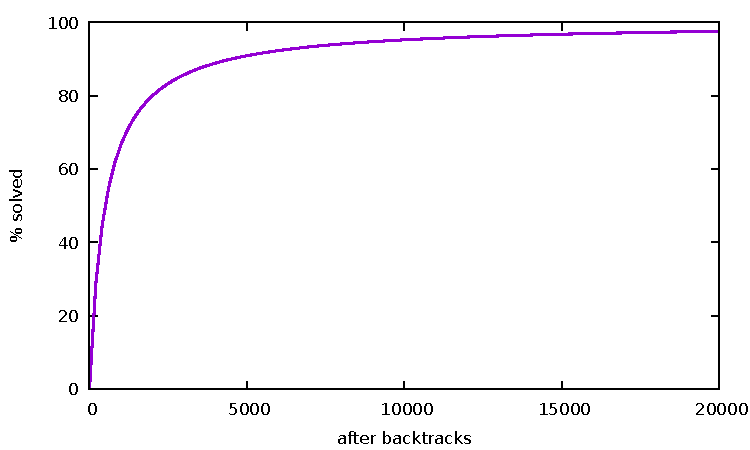
\includegraphics[width=20em]{./long-tail.pdf}}
\item Restarts avoid getting stuck in long tail:
    \begin{itemize}
    \item Restart after $N$ conflicts.
    \item Keep the learnt clauses.
    \item Dynamically grow $N$ exponentially -- otherwise incomplete.
    \end{itemize}
\item $N$ differs a lot between solvers:
    \begin{itemize}
    \item Initial $N$ may vary from high hundreds to low tens.
    \item Trend is to smaller $N$.
    \end{itemize}
\end{itemize}
\end{frame}

\section{Conclusion}

\begin{frame}{Enumerating Models}
Suppose the SAT solver computes a satisfying assignment $I$.

\bigskip
\bigskip
How to find another one?
\end{frame}

\begin{frame}{Satisfiability for $\leq 2$-Clauses}
\begin{thm}{Theorem: complexity of \kSAT2}
\kSAT2 can be solved in polynomial time.
\end{thm}
\begin{itemize}
\item Input: 2-CNF formula $\phi$ of length $n$.
\item Let $\phi^\ast$ be the least set such that
    \begin{itemize}
    \item $\phi \subseteq \phi^\ast$ and
    \item if $(x \lor y), \; (\flip x \lor z) \in \phi^\ast$, \; then $(y \lor z) \in \phi^\ast$.
    \end{itemize}
\item $\phi$ is equivalent to $\phi^\ast$.
\item $\phi$ is unsatisfiable iff $(x \lor x), (\neg x \lor \neg x) \in \phi^\ast$ for some $x$.
\item $|\{x \mid \text{$x$ literal in $\phi$}\}| \leq n$.
\item $|\{(x \lor y, \flip x \lor z) \mid \text{$y, z$ literal in $\phi$}\}| \leq n^2$ for each \rlap{literal $x$.}
\end{itemize}
\end{frame}

\begin{frame}{Benchmarks}
\begin{adjustwidth}{-2em}{-2em}
\begin{tabular}{lrrrrr}
\toprule
Benchmark             & \#Variables & \#Clauses & Naive & WSL    & CDCL\\
\midrule
aim-50-1\_6-yes1-4    &      50 &          80 &   --- & 3\texttimes 10\rlap{\textsuperscript{-3}} & 3\texttimes 10\rlap{\textsuperscript{-4}}\\
uf75-013              &      75 &         325 &   --- & 4\texttimes 10\rlap{\textsuperscript{-4}} & 2\texttimes 10\rlap{\textsuperscript{-4}}\\
pigeon/12             &     156 &         949 &   --- &                                       --- & 2{.0}\\
example2\_gr\_rcs\_w6 &   2,664 &      27,684 &   --- &                                       --- & 3\texttimes 10\rlap{\textsuperscript{-3}}\\
fvp-unsat             &  24,065 &     731,850 &   --- &                                       --- & ---\\
cache\_10             & 227,210 &     879,754 &   --- &                                       --- & 86{.4}\\
\bottomrule
\end{tabular}
\end{adjustwidth}

\bigskip
Execution time (in seconds) of different algorithms:
\begin{itemize}
\item Naive: Slide~\ref{algo:naive}
\item WSL: Slide~\ref{algo:wsl} with watched literal scheme
\item CDCL: Slide~\ref{algo:cdcl} with watched literal scheme, FirstUIP clause \rlap{learning}
\end{itemize}
Timeout after 600 seconds.

\bigskip
Most of the files are from othe 2002 SAT competition.
\end{frame}

\begin{frame}[t]{Pigeonhole Principle}
\bigskip
\textbf{Pigeonhole principle:} $k+1$ pigeons cannot be put in $k$ \rlap{holes.}

\bigskip
\only<-3>{
\begin{align*}
k = \only<1>{1}\only<2>{2}\only<3>{3}: \qquad
&              (h_1 \e {p_1} \only<2->{\lor h_2 \e {p_1} \only<3->{\lor h_3 \e {p_1}}}) \land{}\\
&              (h_1 \e {p_2} \only<2->{\lor h_2 \e {p_2} \only<3->{\lor h_3 \e {p_2}}}) \uncover<2->{\land{}}\\
& \uncover<2->{(h_1 \e {p_3} \only<2->{\lor h_2 \e {p_3} \only<3->{\lor h_3 \e {p_3}}}) \uncover<3->{\land{}}}\\
& \uncover<3->{(h_1 \e {p_4}           \lor h_2 \e {p_4}           \lor h_3 \e {p_4}  ) \phantom{{}\land{}}}\\
\end{align*}
where we assume ${p_i} \neq {p_j}$ for $i \neq j$.
}
\only<4>{
\centering
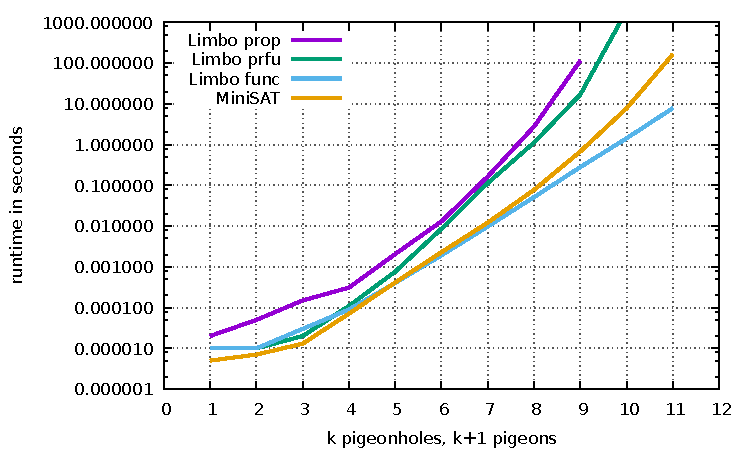
\includegraphics[width=.95\textwidth]{./pigeonhole.pdf}
}
\end{frame}

\begin{frame}{Summary SAT}
\begin{itemize}
\item SAT is provably hard:
    \begin{itemize}
    \item SAT is \red{\NP-complete} -- believed to take exponential time.
    \item All problems in \green{NP can be reduced to SAT} efficiently.\\
    \item SAT is perhaps the best-understood \rlap{problem of complexity theory.}
    \end{itemize}
    \medskip
    \pause
\item SAT is often feasible in practice:
    \begin{itemize}
    \item SAT solvers are far-developed.
    \item Hence SAT is an attractive target for reductions.
    \item Real-world instances often have \blue{easy structure}.
    \item There are small but very hard instances though.
    \end{itemize}
    \medskip
    \pause
\item Key ingredients for a fast SAT solver:
    \begin{itemize}
    \item \blue{Watched-Literal Scheme}
    \item \blue{Clause Learning}
    \item Variable Selection Heuristic
    \item Random Restarts
    \end{itemize}
\end{itemize}
\end{frame}

\section{Beyond SAT}

\begin{frame}{Quantified Boolean Formulas}
Syntax: \; propositional logic \quad $\ex x \phi$ \quad $\fa x \phi$

\bigskip
\pause
Semantics:
\begin{itemize}
\item $x$ is true \;iff\; $x = \TRUE$
\item $\neg \phi$ is true \;iff\; $\phi$ is not true
\item $(\phi_1 \lor \phi_2)$ is true \;iff\; $\phi_1$ or $\phi_2$ is true
\item $(\phi_1 \land \phi_2)$ is true \;iff\; $\phi_1$ and $\phi_2$ are true
\item $\ex x \phi$ is true \;iff\; $\phi^x_\FALSE$ or $\phi^x_\TRUE$ is true
\item $\fa x \phi$ is true \;iff\; $\phi^x_\FALSE$ and $\phi^x_\TRUE$ are true
\end{itemize}
where $\phi^x_y$ is $\phi$ with $x$ replaced by $y$.

\bigskip%
\fly<3-8>{%
\important{Ex.}:~\;~We abbreviate $\FALSE, \TRUE$ by
\renewcommand\TRUE{{\normalfont\textsc{t}}}%
\renewcommand\FALSE{{\normalfont\textsc{f}}}%
$\FALSE, \TRUE$:
\begin{itemize}
\item[] $\fa x \ex y ((\neg x \lor y) \land (x \lor \neg y))$ is true
\uncover<4->{
\item[iff] $\ex y ((\neg \FALSE \lor y) \land (\FALSE \lor \neg y))$ is true \; and\\
      $\ex y ((\neg \TRUE \lor y) \land (\TRUE \lor \neg y))$ is true
}
\uncover<5->{
\item[iff] $\big($\green<8>{$\green<7>{(\green<6>{(\neg \FALSE \lor \FALSE)} \land \green<6>{(\FALSE \lor \neg \FALSE)})}$ or $\red<7>{(\green<6>{(\neg \FALSE \lor \TRUE)} \land \red<6>{(\FALSE \lor \neg \TRUE)})}$ is true$\big)$} \; and\\
      $\big($\green<8>{$\red<7>{(\red<6>{(\neg \TRUE \lor \FALSE)} \land \green<6>{(\TRUE \lor \neg \FALSE)})}$ or $\green<7>{(\green<6>{(\neg \TRUE \lor \TRUE)} \land \green<6>{(\TRUE \lor \neg \TRUE)})}$ is true$\big)$}
}
\end{itemize}
}%
\uncover<9->{%
\important{Note}: \; For propositional $\phi$:
\begin{itemize}
\item $\phi$ is satisfiable \;iff\; $\ex {x_1} \ldots \ex {x_k} \phi$ is true
\item $\phi$ is valid \;iff\; $\fa {x_1} \ldots \fa {x_k} \phi$ is true
\end{itemize}
}%

\uncover<10->{
\bigskip
\pause
\begin{thm}{Theorem: complexity of QBF}
Deciding whether a QBF is true is \PSPACE-complete.
\end{thm}
}
\end{frame}

\begin{frame}{Model Counting}
How many satisfying assignment does a formula have?
\begin{itemize}
\item Exact solvers struggle with huge solution space.
\item Approximative solvers sample solution space.
\item Useful for probabilistic reasoning.
\end{itemize}

\end{frame}

\begin{frame}{Satisfiability Modulo Theories}
Combine SAT solver with a theory solver (e.g., linear equations).

\bigskip
\begin{itemize}
\item $\red<4->{(x + y \geq 3)} \lor \alt<-2>{(x + y \leq 1)}{\green<4->{(-x - y \geq -1)}}$
\item \alt<-2>{$(x < 1) \limp (y < 3)$}{$\blue{(x \geq 1)} \lor \neg \pink{(y \geq 3)}$}
\item<2-> \alt<-2>{$(x < 1) \land (y < 3) \limp (x + y < 3)$}{$\blue{(x \geq 1)} \lor \pink{(y \geq 3)} \lor \neg \red{(x + y \geq 3)}$}
\end{itemize}

\uncover<4->{
\begin{itemize}
\item $\red{p} \lor \green{q}$
\item $\blue{r} \lor \neg \pink{s}$
\item $\blue{r} \lor \pink{s} \lor \neg \red{p}$
\end{itemize}

\begin{itemize}
\item $\flip r, \flip s, \flip p, q$ \; $\Rightarrow$ \; $(x < 1), (y < 3), (x + y < 3)\phantom{, (x + y \leq 1)}$ \; \red{\xmark}
\item $r, s, p, q$                   \; $\Rightarrow$ \; $(x \geq 1), (y \geq 3), (x + y \geq 3), (x + y \leq 1)$ \; \red{\xmark}
\item $r, s, \flip p, q$             \; $\Rightarrow$ \; $(x \geq 1), (y \geq 3), (x + y < 3), (x + y \leq 1)$ \; \green{\cmark}
\end{itemize}
}
\end{frame}

\end{document}

